\let\negmedspace\undefined
\let\negthickspace\undefined
\documentclass[journal,12pt,twocolumn]{IEEEtran}
\usepackage{cite}
\usepackage{amsmath,amssymb,amsfonts,amsthm}
\usepackage{algorithmic}
\usepackage{graphicx}
\usepackage{textcomp}
\usepackage{xcolor}
\usepackage{txfonts}
\usepackage{listings}
\usepackage{enumitem}
\usepackage{mathtools}
\usepackage{gensymb}
\usepackage{comment}
\usepackage[breaklinks=true]{hyperref}
\usepackage{tkz-euclide}
\usepackage{listings}
\usepackage{gvv}
\def\inputGnumericTable{}
\usepackage[latin1]{inputenc}
\usepackage{color}
\usepackage{array}
\usepackage{longtable}
\usepackage{calc}
\usepackage{multirow}
\usepackage{hhline}
\usepackage{ifthen}
\usepackage{lscape}

\newtheorem{theorem}{Theorem}[section]
\newtheorem{problem}{Problem}
\newtheorem{proposition}{Proposition}[section]
\newtheorem{lemma}{Lemma}[section]
\newtheorem{corollary}[theorem]{Corollary}
\newtheorem{example}{Example}[section]
\newtheorem{definition}[problem]{Definition}
\newcommand{\BEQA}{\begin{eqnarray}}
\newcommand{\EEQA}{\end{eqnarray}}
\newcommand{\define}{\stackrel{\triangle}{=}}
\theoremstyle{remark}
\newtheorem{rem}{Remark}
\begin{document}

\bibliographystyle{IEEEtran}
\vspace{3cm}

\title{NCERT Discrete - 11.9.5.8}
\author{EE23BTECH1205 - Avani Chouhan$^{*}$% <-this % stops a space
}
\maketitle
\newpage
\bigskip

\renewcommand{\thefigure}{\theenumi}
\renewcommand{\thetable}{\theenumi}

\vspace{3cm}
\textbf{Question : 11.9.5.8} \\
In a potato race, a bucket is placed at the starting point, which is $5$m from the first potato, and the other potatoes are placed $3$m apart in a straight line. There are ten potatoes in the line.\\
A competitor starts from the bucket, picks up the nearest potato, runs back with it, drops it in the bucket, runs back to pick up the next potato, runs to the bucket to drop it in, and she continues in the same way until all the potatoes are in the bucket. What is the total distance the competitor has to run?\\

\solution
The distance covered forms an AP with give parameters \\
 \begin{tabular}{|c|c|c|}
    \hline
    \textbf{Parameter} & \textbf{Value} & \textbf{Description} \\
    \hline
    $x(0)$ & $10$ & First term \\
    \hline
    $d$ & $6$ & Common difference \\
    \hline 
    $x(n)$ & $10+6n$ & general term \\
    \hline 
\end{tabular}

 
 \begin{align}
 x(n) &= x(0)+nd
 \end{align}
Applying Z transform:
\begin{align}
    X(z) &=\frac{10}{1-z^{-1}} + \frac{6z^{-1}}{(1-z^{-1})^2} 
    \quad \abs{z}>\abs1
\end{align}

For AP, the sum of first n+1 terms can be written as :
\begin{align}
	 y(n)&=x(n)*u(n) \\
	 Y(z) &= X(z)U(z)
\end{align}  
From equation \eqref{eq:11.9.5.26.2}:
\begin{align}
	&=\frac{10}{(1-z^{-1})^2} + \frac{6z^{-1}}{(1-z^{-1})^3}
	\quad \abs{z}>\abs1
\end{align}
Using contour integration to find inverse Z transform:
\begin{align}
	y(n) &= \frac{1}{2\pi j} \oint_C Y(z) z^{n-1} dz\\
	&= \frac{1}{2\pi j} \oint_C [ \frac{10}{(1-z^{-1})^2} + \frac{6z^{-1}}{(1-z^{-1})^3} ]z^{8} \, dz
\end{align}
The sum of the terms of the sequence is computed using the residue theorem, expressed as $R_i$, which represents the residue of the Z-transform at $ z=1 $ for the expression $ Y(z) $.
\begin{align}
	R_i=R_1 + R_2
\end{align}
 $R_1$ and $R_2$ are residues calculated at the poles of the Z-transform.
\begin{align}
		R_1 &= \frac{1}{{(2-1)!}} . \frac{d (10z^{10})}{dz} |_{z=1} \\
	&=10*10=100
\end{align}
\begin{align}
	R_2 &= \frac{1}{{(3-1)!}} . \frac{d^2(6z^{10})}{dz^2} |_{z=1} \\
	&= \frac{6}{2}(10)(9) = 270
\end{align}
The sum of terms is given by $R_i$:
 \begin{align}
100 + 270 = 370
\end{align}
\begin{figure}
    \centering
    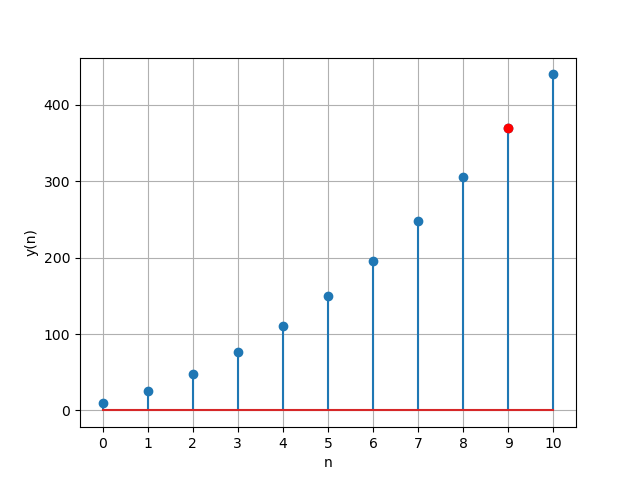
\includegraphics[width=\columnwidth]{figs/plot2.png}
    \caption{Stem plot of y(n)}
    \label{fig:11.9.5.8fig1}
\end{figure}
\end{document}
